\documentclass{lug}

\usepackage{fontawesome}
\usepackage{etoolbox}
\usepackage{etoolbox}
\usepackage{textcomp}
\usepackage[nodisplayskipstretch]{setspace}
\usepackage{xspace}

\AtBeginEnvironment{minted}{\singlespacing\fontsize{10}{10}\selectfont}

\makeatletter
\patchcmd{\beamer@sectionintoc}{\vskip1.5em}{\vskip0.5em}{}{}
\makeatother

\newcommand{\pmidg}[1]{\parbox{\widthof{#1}}{#1}}
\newcommand{\splitslide}[4]{
    \noindent
    \begin{minipage}{#1 \textwidth - #2 }
        #3
    \end{minipage}%
    \hspace{ \dimexpr #2 * 2 \relax }%
    \begin{minipage}{\textwidth - #1 \textwidth - #2 }
        #4
    \end{minipage}
}

\title{Filesystems}
\author{Sumner Evans and Sam Sartor}
\institute{Mines Linux Users Group}

\begin{document}

\section{Introduction}

\begin{frame}{What are Filesystems?}
    \begin{itemize}
        \item Filesystems manage the storage and retrieval of files from storage
            media.
        \item Filesystems are an abstraction layer between storage media (SSDs,
            HDDs, disk drives, even tape drives).
        \item Filesystems exist on \textit{partitions}, physically contiguous
            segments of the disk.
    \end{itemize}
\end{frame}

\begin{frame}{Filesystems are Responsible for\ldots}
    \begin{itemize}
        \item \textbf{Space management:} filesystems allocate and manage space
            in discrete chunks. Filesystems must keep track of what data is
            stored at each chunk.
        \item \textbf{Filenames:} identify a storage location in the file
            system. Can be case sensitive (ext4) or case insensitive (HFS,
            NTFS).
        \item \textbf{Directories (folders):} group files into separate
            collections. Modern filesystems allow arbitrary nesting of
            directories.
        \item \textbf{Metadata:} filesystems store book-keeping information
            about their contents (e.g. file sizes, last accessed date, owner and
            permissions, etc.).
        \item \textbf{Access Control:} prevent unauthorized access to files on
            disk.
        \item \textbf{Data Integrity:} filesystems must be resilient to failure,
            some are better at this than others.
    \end{itemize}
\end{frame}

% \section{History of Filesystems}
% \begin{frame}{The First Filesystems}
%     \splitslide{0.60}{1em}{
%         The filesystem was originally thought of as part of the operating
%         system.

%         One of the first filesystems that had a name was DECTape. DECTape stored
%         an astoundingly small 184 kilobytes (kilo, not mega) of data per tape on
%         the PDP-8.
%     }{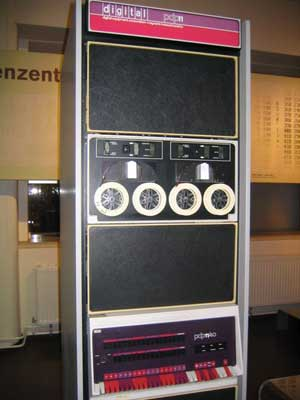
\includegraphics[width=0.4\textheight]{./graphics/dectape.jpg}}
% \end{frame}

% \begin{frame}{CM/P $\rightarrow$ FAT}

% \end{frame}

\section{Current Filesystems}

\section{Linux}
\begin{frame}{ext4}
\end{frame}

\section{Windows \& mac}
\begin{frame}{NTFS}
\end{frame}

\begin{frame}{HFS and HFS+}
    Apple has made a ton of filesystems with varying degrees of terribleness.
    \begin{itemize}
        \item \textbf{HFS:} Hierarchical File System --- Introduced in 1985 with
            the first Apple computer with a hard drive. Had a limitation of
            65,535 files and every file had to take up at least 1 / 65,535th of
            the disk.

        \item \textbf{HFS+:} Released in 1998 to fix some of the issues with
            HFS. the core of the filesystem uses case-insensitive NFD Unicode
            strings, which led Linus Torvalds to say that ``HFS+ is probably the
            worst file-system ever''.
    \end{itemize}
\end{frame}

\begin{frame}{APFS}
    \textbf{APFS:} Apple Filesystem --- Introduced in June 2016 to replace HFS+
    and is optimized for SSDs. It fixes some of the problems of HFS+. Basically
    it replicates the work of other modern filesystems which are actually
    maintained by large communities.

    Apple forcibly upgraded all computers to APFS in macOS High Sierra.
\end{frame}

\section{Flashdrives}
\begin{frame}{FAT32}
\end{frame}

\begin{frame}{Other Options}
\end{frame}

\section{Alternative Filesystems}
\begin{frame}{Btrfs}
    \textbf{B}-\textbf{tr}ee \textbf{f}ile \textbf{s}ystem (Btrfs) pronounced
    ``Butter FS'' or ``better FS'' or ``b-tree FS'' was developed starting in
    2007 by Oracle.

    \textbf{Pros}
    \begin{itemize}
        \item Copy on Write
        \item Mostly self-healing
        \item Can convert from \texttt{etx*} to Btrfs
    \end{itemize}

    \textbf{Cons}
    \begin{itemize}
        \item It's being depricated by Oracle. RHEL 7.4 includes it, but they
            are transitioning away. The SUSE project will still use and maintain
            it.
    \end{itemize}
\end{frame}

% \begin{frame}{XFS}

% \end{frame}

\begin{frame}{ZFS}
\end{frame}

\begin{frame}{TFS}
\texttt{TFS} is a work-in-progress filesystem for the Redox operating system.
Intended as a modern alternative to ZFS, the feature list is mouth-watering.

\textbf{Pros}\begin{itemize}
    \item Concurrent \& non-blocking
    \item Lightweight full-disk compression
    \item Zero-overhead revision history
    \item Automatic corruption detection
    \item $O(1)$ recursive directory copies
    \item Designed for solid state drives
    \item Perfectly resilient to power loss 
\end{itemize}

\textbf{Cons}\begin{itemize}
    \item Not fully implemented yet
\end{itemize}
\end{frame}

\section{Network Filesystems}
\begin{frame}{What is a network filesystem?}
\begin{center}
    You can access remote storage devices over the internet using a
    \emph{network filesystem}.
\end{center}
\end{frame}

\begin{frame}{NFS}
\end{frame}

\begin{frame}{Samba}
\end{frame}

\section{Virtual Filesystems}
\begin{frame}{What is a virtual filesystem?}
\begin{center}
    A \emph{virtual filesystem} is an abstraction layer which converts some
    other source of data to a filesytem-like structure.

    Colloquially, any filesystem that is not stored on disk is called a virtual
    filesystem. These can be procedural or abstract other kinds of devices.
\end{center}
\end{frame}

\begin{frame}{tmpfs}
    A *Nix \texttt{tmpfs} is a filesystem stored in RAM. They appear as mounted
    filesystems, but are stored in volitile memory.  By default, the
    \texttt{/tmp} directory is a \texttt{tmpfs}.

    \textbf{Pros}
    \begin{itemize}
        \item Useful for storing temporary files such as downloads and temporary
            files for programs.
        \item Saves unnecessary disk I/O.
        \item Security: you can use it to temporarily store sensitive, decrypted
            files so that the decrypted data is never written to disk.
    \end{itemize}

    \textbf{Cons}
    \begin{itemize}
        \item Everything in a \texttt{tmpfs} will be deleted on reboot since RAM
            is volitile.
    \end{itemize}
\end{frame}

\begin{frame}{procfs}
    In *Nix, everything is a file. This includes things such as process
    information. The way to access this data is through the \texttt{proc}
    filesystem which provides a convenient and standardized method for
    dynamically accessing process data held in the kernel.

    In Linux, \texttt{procfs} contains more than just process information
    including memory information, network utilization statistics, etc.
\end{frame}

\begin{frame}{FUSE}
Filesystem in Userspace (FUSE) is an interface for creating filesystems
without writing any kernel-level code, which makes it incredibly useful for
creating virtual filesystems. It is an available in Linux, FreeBSD, OpenBSD,
NetBSD, OpenSolaris, Minix 3, Android, and macOS.

\texttt{libfuse}\ldots \begin{itemize}
    \item is a C library
    \item provides a high-level interface for FUSE
    \item makes creating new filesystems really easy 
    \item has bindings for Python, Rust, etc.
\end{itemize}
\end{frame}

\begin{frame}{sshfs}
\texttt{sshfs} is a network filesystem implemented through libfuse. You can
use it to mount remote directories via ssh.

\textbf{Pros}\begin{itemize}
    \item Very easy \& quick to setup (one command)
    \item Remote machine only needs ssh installed
\end{itemize}

\textbf{Cons}\begin{itemize}
    \item Intended to be temporary
    \item Generally slower than NFS
\end{itemize}
\end{frame}

\section{Configuration/maintenance}

\begin{frame}{\ldots}
\end{frame}

\begin{frame}[standout]
    \Huge
    Questions?
\end{frame}

\begin{frame}{References}
    \begin{itemize}
        \item \url{https://en.wikipedia.org/wiki/File_system}
        \item \url{http://www.tldp.org/LDP/sag/html/filesystems.html}
        \item \url{https://arstechnica.com/gadgets/2008/03/past-present-future-file-systems/2/}
    \end{itemize}
\end{frame}

\end{document}
